\chapter{Control de un Crazyflie}

Dado un conocimiento básico de Paparazzi, este capítulo se centra en la 
implementación de los algoritmos de control para un sólo Crazyflie. 
Se realizarán implementaciones parcialmente agnósticas del posicionamiento entre drones,
al no ser necesaria la coordinación entre drones. 

Se entenderá el funcionamiento de un algoritmo GVF y se verá su 
implementación en Paparazzi para el Crazyflie, terminando con un buen control de este.

%%%%%%%%%%%%%%%%%%%%%%%%%%%%%%%%%%%%%%%%%%%%%%%%%%%%%%%%%%%%%%%%%%%%%%%%%%%%%%%%%%%%%%%%%%%%%%%%%%%%%%%%%%%%%%%%%
%%%%%%%%%%%%%%%%%%%%%%%%%%%%%%%%%%%%%%%%%%%%%%%%%%%%%%%%%%%%%%%%%%%%%%%%%%%%%%%%%%%%%%%%%%%%%%%%%%%%%%%%%%%%%%%%%
%%%%%%%%%%%%%%%%%%%%%%%%%%%%%%%%%%%%%%%%%%%%%%%%%%%%%%%%%%%%%%%%%%%%%%%%%%%%%%%%%%%%%%%%%%%%%%%%%%%%%%%%%%%%%%%%%

\section{Control básico}

Previo a conseguir control con algoritmos avanzados, se debe conseguir \textit{hovering}, 
es decir, que el dron flote estático a cierta altura. 
Debido a que la implementación de Paparazzi actual esta enfocada a control manual con mando, 
el PID no está debidamente ajustado. 
Conseguir hovering se reduce a un correcto ajuste del PID vertical y horizontal, 
al estar el control por PID ya implementado en el firmware del Crazyflie.

%%%%%%%%%%%%%%%%%%%%%%%%%%%%%%%%%%%%%%%%%%%%%%%%%%%%%%%%%%%%%%%%%%%%%%%%%%%%%%%%%%%%%%%%%%%%%%%%%%%%%%%%%%%%%%%%%
%%%%%%%%%%%%%%%%%%%%%%%%%%%%%%%%%%%%%%%%%%%%%%%%%%%%%%%%%%%%%%%%%%%%%%%%%%%%%%%%%%%%%%%%%%%%%%%%%%%%%%%%%%%%%%%%%
%%%%%%%%%%%%%%%%%%%%%%%%%%%%%%%%%%%%%%%%%%%%%%%%%%%%%%%%%%%%%%%%%%%%%%%%%%%%%%%%%%%%%%%%%%%%%%%%%%%%%%%%%%%%%%%%%

\subsection{PID en Paparazzi}

Paparazzi reduce el control de un rotorcraft a dos controladores PID: \textbf{uno vertical (eje Z) y otro horizontal (plano y ejes XY)}. 
El control PID en Paparazzi no difiere mucho de un control PID estándar, no obstante, cabe destacar una leve diferencia en el control PID vertical:

\begin{equation}
    m(t) = m_h + K_p e(t) + K_i \int_{0}^{t} e(t)dt + K_d \frac{de(t)}{dt}
\end{equation}

Donde:

\begin{itemize}
    \item $m(t)$ es el throttle (velocidad de los motores de 0 a 100\%) respecto al tiempo
    \item $m_h$ es el \textit{Nominal Hover Throttle}, es decir, el valor mínimo de throttle deseado. 
    Se fija a un valor muy levemente por debajo del valor mínimo para que un Crazyflie despegue. 
    Se encontró que un Crazyflie despega con un throttle de \textbf{entre 65\% y 70\%}
    \item $e(t)$ es el error respecto a la altura deseada
\end{itemize}

Nuestra principal diferencia, como se puede observar, reside en el Nominal Hover Throttle. 
Con este valor se consigue que el dron parta de un valor inicial de throttle con sentido, 
es decir, que le permita despegar del suelo. 
La siguiente figura ilustra perfectamente la idea recién explicada:

\begin{figure}[h]
    \centering
    \includegraphics[width=0.95\textwidth]{img/fig/fig3.1-vertical-pid.png}
    \caption{Comparativa entre la altura conseguida por el PID y el throttle respecto al mismo tiempo. 
    En \textcolor{blue}{azul}, el throttle, en \textcolor{red}{rojo}, la altura.
    Notación: $h(t)$ altura respecto al tiempo, $h_d$ altura deseada, 
    $m_h$ es el nominal hover throttle y $m_d$ throttle para altura deseada}
    \label{fig:vertical-pid}
\end{figure}

%%%%%%%%%%%%%%%%%%%%%%%%%%%%%%%%%%%%%%%%%%%%%%%%%%%%%%%%%%%%%%%%%%%%%%%%%%%%%%%%%%%%%%%%%%%%%%%%%%%%%%%%%%%%%%%%%
%%%%%%%%%%%%%%%%%%%%%%%%%%%%%%%%%%%%%%%%%%%%%%%%%%%%%%%%%%%%%%%%%%%%%%%%%%%%%%%%%%%%%%%%%%%%%%%%%%%%%%%%%%%%%%%%%
%%%%%%%%%%%%%%%%%%%%%%%%%%%%%%%%%%%%%%%%%%%%%%%%%%%%%%%%%%%%%%%%%%%%%%%%%%%%%%%%%%%%%%%%%%%%%%%%%%%%%%%%%%%%%%%%%

\subsection{Metodología para ajuste del PID}

Idealmente, se puede automatizar el ajuste de un PID con un \textit{testbench} para drones,
que permite automáticamente ajustar los valores más precisos de manera automática. 
No obstante, las capacidades de telemetría de Paparazzi permiten diagnosticar manualmente el 
resultado de un control PID. En general, se siguió la siguiente metodología:

\begin{itemize}
    \item \textbf{Ajuste del control proporcional:} se ajusta el control proporcional hasta que se consiga que el dron despegue hasta una altura no muy lejana del objetivo, con error constante.
    \item \textbf{Ajuste del control integral:} se añade lentamente constante integral hasta que se consiga ver que esta compensa los errores del proporcional y oscila alrededor de la altura deseada.
    \item \textbf{Ajuste del control derivativo:} se ajusta la constante derivativa hasta reducir el overshoot inicial lo suficiente sin que desestabilice el control PI.
\end{itemize}

Para averiguar el nominal hover throttle se hizo a ensayo y error, debido a que es fácil averiguarlo: probar numeros de 0 a 1 (0 a 100\%) hasta que el dron de pequeños saltos.

%%%%%%%%%%%%%%%%%%%%%%%%%%%%%%%%%%%%%%%%%%%%%%%%%%%%%%%%%%%%%%%%%%%%%%%%%%%%%%%%%%%%%%%%%%%%%%%%%%%%%%%%%%%%%%%%%
%%%%%%%%%%%%%%%%%%%%%%%%%%%%%%%%%%%%%%%%%%%%%%%%%%%%%%%%%%%%%%%%%%%%%%%%%%%%%%%%%%%%%%%%%%%%%%%%%%%%%%%%%%%%%%%%%
%%%%%%%%%%%%%%%%%%%%%%%%%%%%%%%%%%%%%%%%%%%%%%%%%%%%%%%%%%%%%%%%%%%%%%%%%%%%%%%%%%%%%%%%%%%%%%%%%%%%%%%%%%%%%%%%%

\subsection{Hovering}

En la siguiente tabla tenemos los valores del PID para el controlador vertical. 
Como en cualquier control de tipo PID, tenemos las constantes proporcionales, derivativas e integrales.
Se añade en este caso el \textit{nominal hover throttle}, como bien se ha explicado previamente.

\begin{table}[h]
\centering
\begin{tabular}{l|c}
    \multicolumn{1}{c|}{\textbf{Variable}} & \textbf{Valor} \\ \hline
    $K_p$                       & 175        \\
    $K_i$                       & 30         \\
    $K_d$                       & 70         \\
    $m_h$                       & 0,625       
\end{tabular}
    \caption{Valores PID vertical}
    \label{tab:vertical_pid}
\end{table}

Paralelamente, tenemos en la siguiente tabla los valores para el PID horizontal, 
que se ocupa de evitar que el Crazyflie se mueva en los ejes X e Y.

\begin{table}[h]
\centering
\begin{tabular}{l|c}
    \multicolumn{1}{c|}{\textbf{Variable}} & \textbf{Valor} \\ \hline
    $K_p$   & 50        \\
    $K_i$   & 20        \\
    $K_d$   & 125      
\end{tabular}
    \caption{Valores PID horizontal}
    \label{tab:horizontal_pid}
\end{table}

Con ambos PID bien ajustados, se consigue que el dron se pueda mantener estático a una altura dada:

\begin{figure}[h]
    \centering
    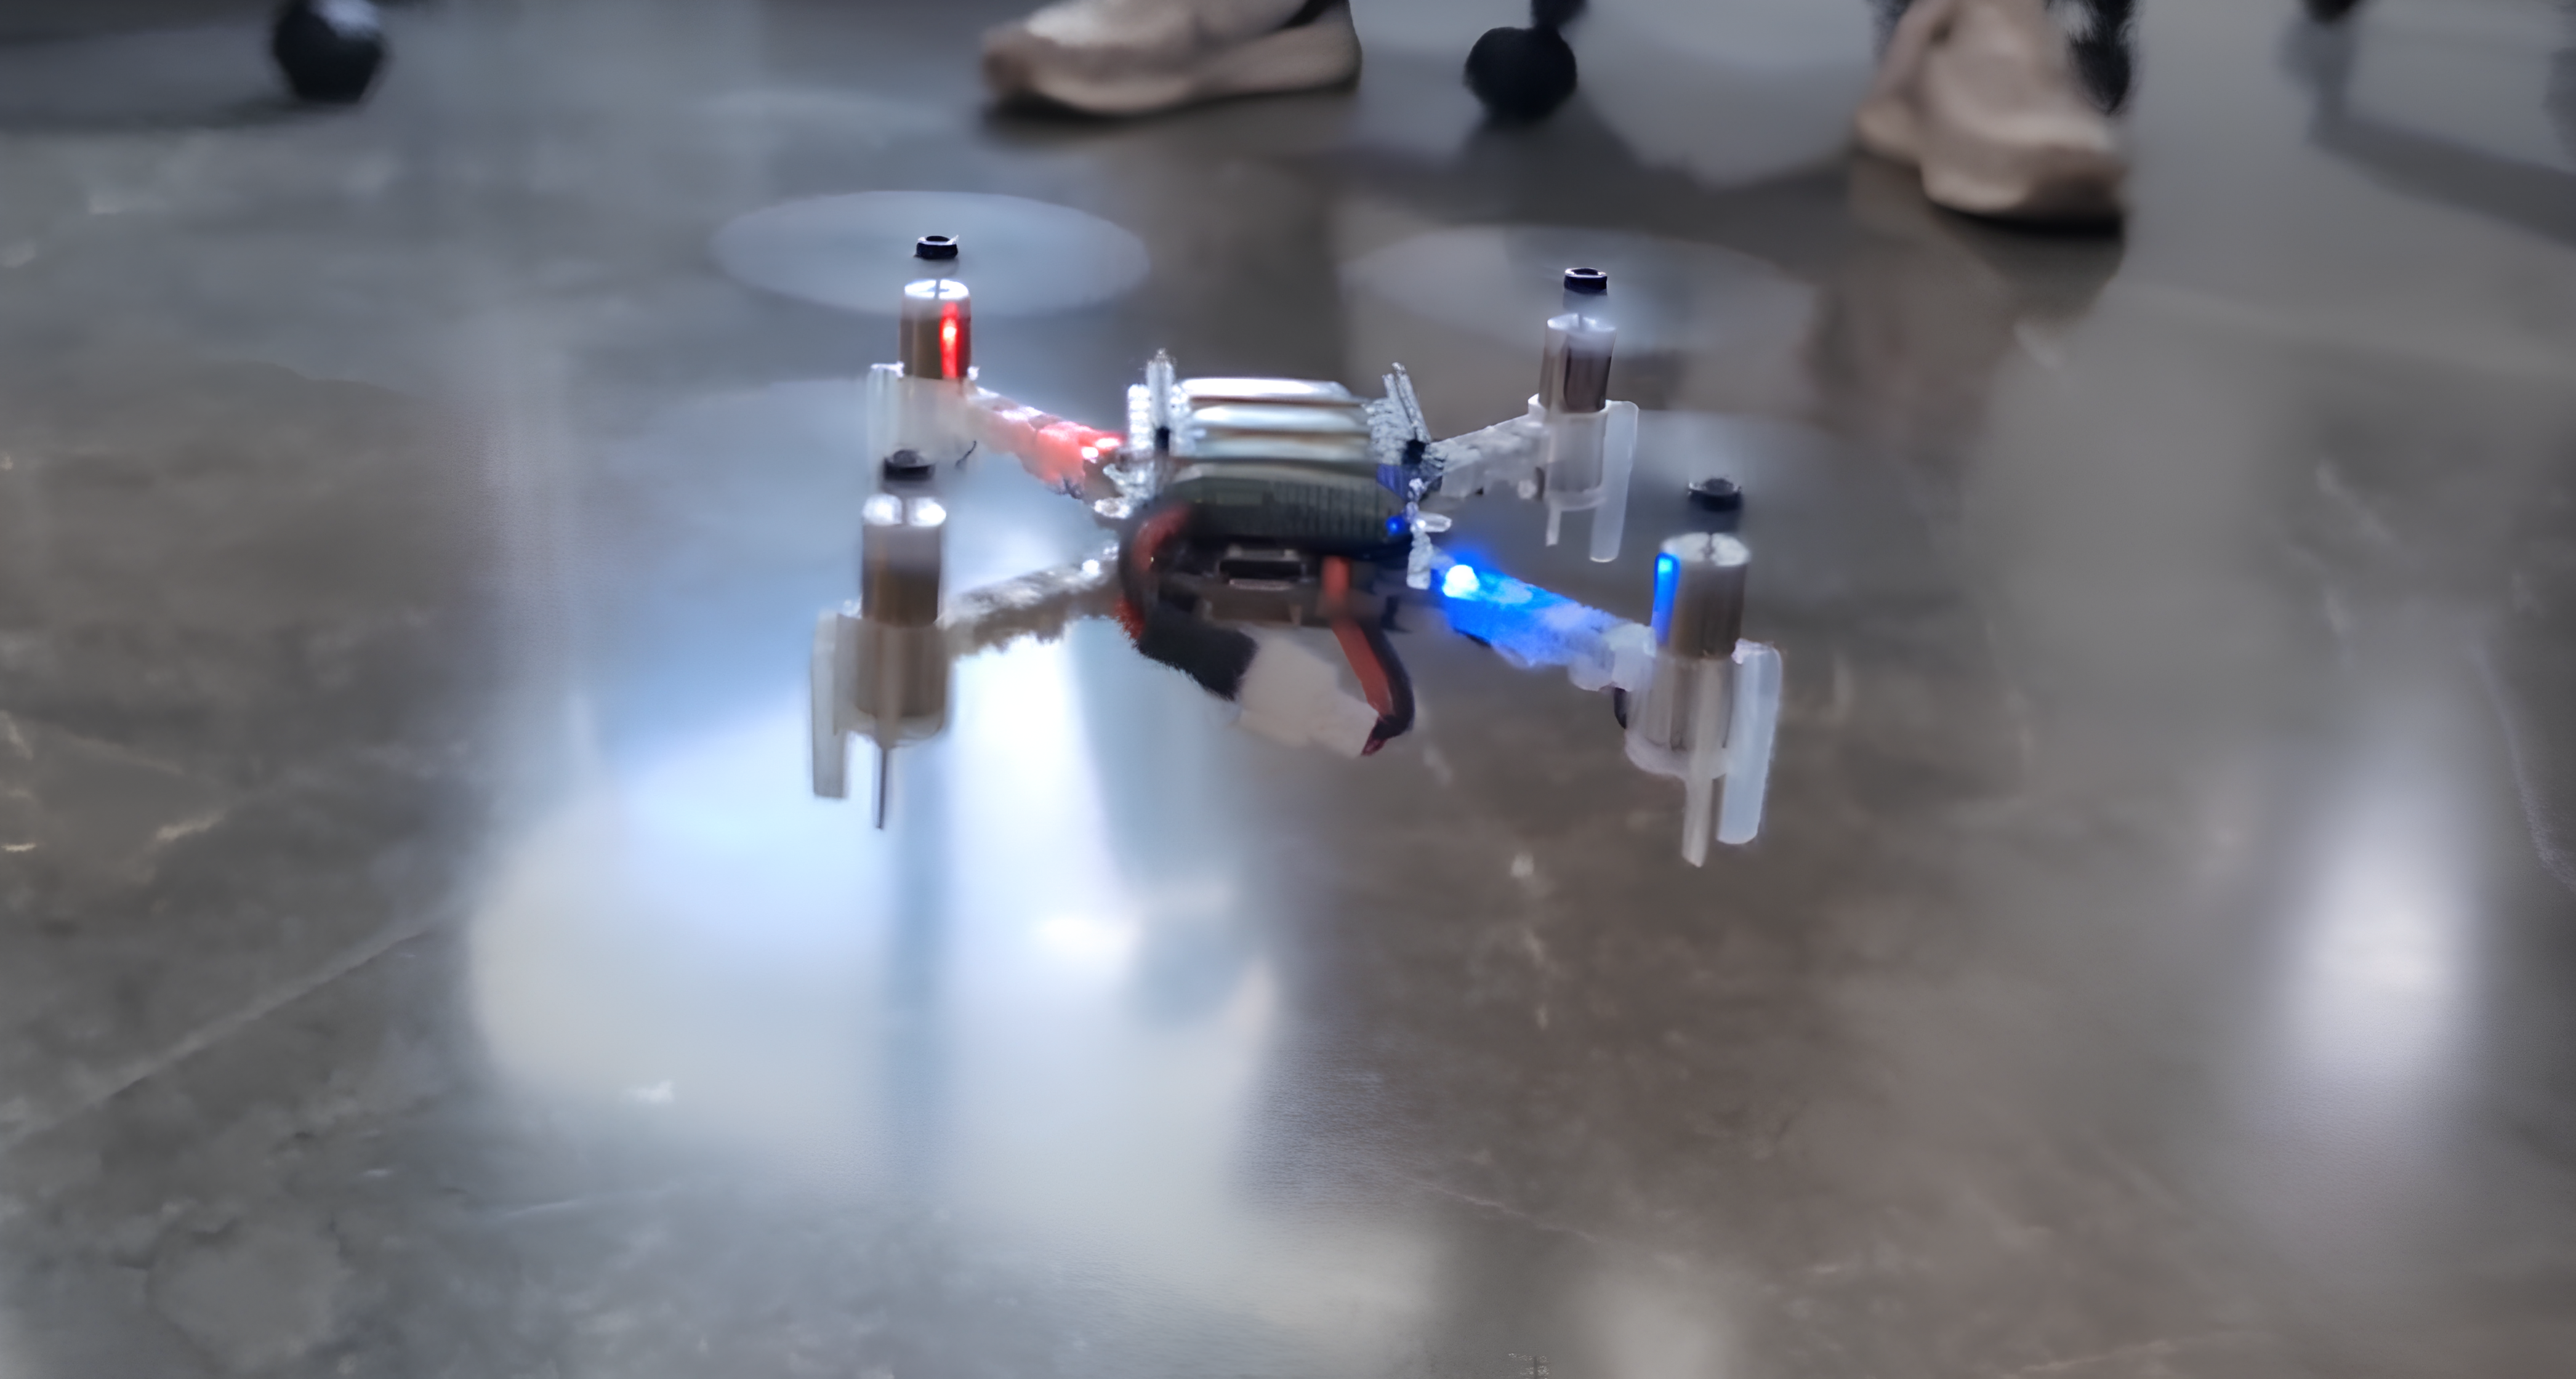
\includegraphics[width=0.7\textwidth]{img/fig/fig3.2-hovering-crazyflie.png}
    \caption{Crazyflie haciendo hovering}
    \label{fig:hovering-crazyflie}
\end{figure}

%%%%%%%%%%%%%%%%%%%%%%%%%%%%%%%%%%%%%%%%%%%%%%%%%%%%%%%%%%%%%%%%%%%%%%%%%%%%%%%%%%%%%%%%%%%%%%%%%%%%%%%%%%%%%%%%%
%%%%%%%%%%%%%%%%%%%%%%%%%%%%%%%%%%%%%%%%%%%%%%%%%%%%%%%%%%%%%%%%%%%%%%%%%%%%%%%%%%%%%%%%%%%%%%%%%%%%%%%%%%%%%%%%%
%%%%%%%%%%%%%%%%%%%%%%%%%%%%%%%%%%%%%%%%%%%%%%%%%%%%%%%%%%%%%%%%%%%%%%%%%%%%%%%%%%%%%%%%%%%%%%%%%%%%%%%%%%%%%%%%%

\section{Algoritmos GVF}

Entre la variedad de algoritmos de control que se puede implementar, 
se ha elegido un algoritmo GVF (\textit{Guidance Vector Field}).
Este tipo de algoritmo permite recorrer trayectorias en 2D
mediante la creación de un campo vectorial que indíca velocidad y trayectoria 
del vehículo en un punto dado. 
La base matemática de este algoritmo permite bajo consumo de recursos 
(ideal en sistemas empotrados como el Crazyflie) y adaptabilidad a cualquier figura 2D representable matemáticamente.

%%%%%%%%%%%%%%%%%%%%%%%%%%%%%%%%%%%%%%%%%%%%%%%%%%%%%%%%%%%%%%%%%%%%%%%%%%%%%%%%%%%%%%%%%%%%%%%%%%%%%%%%%%%%%%%%%
%%%%%%%%%%%%%%%%%%%%%%%%%%%%%%%%%%%%%%%%%%%%%%%%%%%%%%%%%%%%%%%%%%%%%%%%%%%%%%%%%%%%%%%%%%%%%%%%%%%%%%%%%%%%%%%%%
%%%%%%%%%%%%%%%%%%%%%%%%%%%%%%%%%%%%%%%%%%%%%%%%%%%%%%%%%%%%%%%%%%%%%%%%%%%%%%%%%%%%%%%%%%%%%%%%%%%%%%%%%%%%%%%%%

\subsection{Fundamentos matemáticos}

Como bien se ha explicado previamente, un algoritmo GVF trata de recorrer 
un camino o trayectoria mediante un campo vectorial. 
Matemáticamente, podemos definir un camino $\mathcal{P} \subseteq \mathds{R}^2$
donde $\varphi(p) : \mathds{R}^2 \rightarrow \mathds{R}$
mediante la siguiente ecuación implícita:

\begin{equation}
    \mathcal{P} := \{ p : \varphi(p) = 0\}
\end{equation}

Esta representación, extraída de \cite{gvf-hector} permite ocupar todo el 
plano $\mathds{R}^2$ mediante las curvas de nivel $\{ p : \varphi(p) = c\}$, 
donde la curva que verifica $c = 0$ es la deseada. Con esta representación, a su vez, 
podemos representar el error de distancia (no tiene porque coincidir con la distancia euclídea)
del vehículo respecto a la curva deseada como:

\begin{equation}
    e(p) := \varphi(p) \in \mathds{R}
\end{equation}

Este error, nos permite variar las componentes de un vector de forma que podamos, 
en función de como de grande sea $e(p)$, incrementar o decrementar la \textit{agresividad} 
con la cual el vehículo se aproximará a la curva de nivel deseada. 
Ello, junto a una constante $k_e$ que permitirá variar la agresividad general, concluye 
en el siguiente campo vectorial de guiado propuesto por los autores de \cite{gvf-hector}:

\begin{equation} \label{eq: GVF}
    \dot{p}_d := \tau(p) - k_e e(p) n(p)
\end{equation}

Donde $\dot{p}_d$ es el vector de velocidad deseada, $\tau(p)$ es la tangente de este vector y
$n(p)$ es la componente normal del mismo vector. La siguiente figura explica gráficamente
todo lo explicado hasta ahora:

\begin{figure}[h]
    \centering
    \includegraphics[width=0.7\textwidth]{img/fig/fig3.3-gvf-diagram.png}
    \caption{Representación gráfica de un vehículo bajo el efecto de un GVF. 
    Imagen extraída de \cite{tfm-jesus} y basado en \cite{gvf-hector}.}
    \label{fig:gvf-diagram}
\end{figure}

En esta figura se debe entender también lo siguiente:

\begin{itemize}
    \item $p^*$ es el punto en el plano donde se encuentra el vehículo.
    \item $\dot p$ es la velocidad actual del vehículo.
    \item $\mathcal{O}_N$ es el origen de coordenadas.
    \item $\hat{\dot{p}}_d$ es el vector con módulo normalizado a la unidad (ocasionalmente interesa solo dirección y sentido del vector) de la velocidad deseada.
    \item Tanto $n$ como $\tau$ son calculadas mediante $\nabla\varphi(p^*)$.
\end{itemize}

Como podemos observar en la figura, el resultado $\dot p_d$ tiende hacia la curva 
$\varphi(p) = 0$, es decir, el camino deseado $\mathcal{P}$. 
Es intuitivo observar que, variando la constante $k_e$ y en función de la 
curva de nivel $e$, el resultado de $\dot p_d$ será más normal (perpendicular) 
respecto al camino deseado $\mathcal{P}$, aumentando la previamente llamada agresividad.

%%%%%%%%%%%%%%%%%%%%%%%%%%%%%%%%%%%%%%%%%%%%%%%%%%%%%%%%%%%%%%%%%%%%%%%%%%%%%%%%%%%%%%%%%%%%%%%%%%%%%%%%%%%%%%%%%
%%%%%%%%%%%%%%%%%%%%%%%%%%%%%%%%%%%%%%%%%%%%%%%%%%%%%%%%%%%%%%%%%%%%%%%%%%%%%%%%%%%%%%%%%%%%%%%%%%%%%%%%%%%%%%%%%
%%%%%%%%%%%%%%%%%%%%%%%%%%%%%%%%%%%%%%%%%%%%%%%%%%%%%%%%%%%%%%%%%%%%%%%%%%%%%%%%%%%%%%%%%%%%%%%%%%%%%%%%%%%%%%%%%

\subsection{Algoritmos GVF para rotorcrafts}

Aunque GVF se puede aplicar a cualquier vehículo, los autores de \cite{gvf-hector}
continuan aportando una solución específica para un \textit{fixedwing UAV} 
el cual solo puede modificar sus ángulos de \textit{roll} y \textit{pitch} 
haciendo un movimiento usando la \textbf{velocidad angular ($\omega$)}. 

Por contraparte, un rotorcraft puede modificar su \textit{yaw} y 
puede realizar movimientos más bruscos debido a su capacidad de moverse lateralmente, 
permitiendo mucho mejor control en general. 
Se propone utilizar las \textbf{velocidades en los ejes X e Y} para control de los motores del dron,
ya que las velocidades son ya calculadas en GVF, 
se consigue una aplicación directa de una de las variables ya calculadas. 

Paparazzi incluye un algoritmo de control llamado \textbf{INDI} (\textit{Incremental Nonlinear Dynamic Inversion})
\cite{indi-paparazzi}
que se ocupa del control de forma transparente en base a una posición, velocidad o aceleración dada. 
Gracias a este algoritmo, una vez calculada la aceleración deseada en GVF 
podemos cambiar una variable en el código para que INDI se ocupe de controlar los
motores del dron para conseguir el efecto deseado. 

Debido a la flexibilidad de INDI, se podría haber usado posición o aceleración en vez de velocidad,
pero se usó la velocidad al ser lo más intuitivo y ser un prerrequisito ya calculado para GVF.

%%%%%%%%%%%%%%%%%%%%%%%%%%%%%%%%%%%%%%%%%%%%%%%%%%%%%%%%%%%%%%%%%%%%%%%%%%%%%%%%%%%%%%%%%%%%%%%%%%%%%%%%%%%%%%%%%
%%%%%%%%%%%%%%%%%%%%%%%%%%%%%%%%%%%%%%%%%%%%%%%%%%%%%%%%%%%%%%%%%%%%%%%%%%%%%%%%%%%%%%%%%%%%%%%%%%%%%%%%%%%%%%%%%
%%%%%%%%%%%%%%%%%%%%%%%%%%%%%%%%%%%%%%%%%%%%%%%%%%%%%%%%%%%%%%%%%%%%%%%%%%%%%%%%%%%%%%%%%%%%%%%%%%%%%%%%%%%%%%%%%

\subsection{Limitaciones de GVF sin posicionamiento}

Sin añadir nada a un Crazyflie, las únicas variables que este puede calcular son la aceleración en los ejes X, Y y Z, 
la presión con un barómetro (que permite hacer aproximación de la altura) y
los ángulos de roll, pitch y yaw mediante la IMU que posee \cite{imu-wikipedia}. 

Gracias a la diversas capacidades de Paparazzi, este contiene un módulo llamado \textbf{INS} (del inglés, \textit{Inertial Navigation System}), 
que permite un cálculo aproximado de la velocidad y posición integrando la aceleración.
Desafortunadamente, la naturaleza de este algoritmo y de las operaciones de punto flotante que utiliza, 
acumulan error respecto al tiempo que no se puede corregir sin otro sistema de posicionamiento como el GPS.

Como solución, se va a utilizar uno de los módulos de Bitcraze para el Crazyflie llamado \textbf{Flow Deck v2} \cite{flow-deck}.
Este módulo contiene dos sensores esenciales: 

\begin{itemize}
    \item \textbf{Altímetro:} que sustituye las medidas aproximadas del barómetro por unas de mucha mayor precisión.
    \item \textbf{Opticflow:} cámara que permite detectar velocidades en X e Y al estar mirando hacia el suelo. Necesita que el suelo tenga textura, pero es mucho mas precisa que integrar la aceleración dada por la IMU.
\end{itemize}

\begin{figure}[h]
    \centering
    \includegraphics[width=0.4\textwidth]{img/fig/fig3.4-flow-deck.jpg}
    \caption{Flow Deck V2 de Bitcraze}
    \label{fig:flow-deck}
\end{figure}

De esta forma, aunque se sigue manteniendo el error por posición (aun se necesita integrar la velocidad, para conseguir posición),
la velocidad y la altura (imprescindibles para realizar GVF) ahora son de mayor precisión.

%%%%%%%%%%%%%%%%%%%%%%%%%%%%%%%%%%%%%%%%%%%%%%%%%%%%%%%%%%%%%%%%%%%%%%%%%%%%%%%%%%%%%%%%%%%%%%%%%%%%%%%%%%%%%%%%%
%%%%%%%%%%%%%%%%%%%%%%%%%%%%%%%%%%%%%%%%%%%%%%%%%%%%%%%%%%%%%%%%%%%%%%%%%%%%%%%%%%%%%%%%%%%%%%%%%%%%%%%%%%%%%%%%%
%%%%%%%%%%%%%%%%%%%%%%%%%%%%%%%%%%%%%%%%%%%%%%%%%%%%%%%%%%%%%%%%%%%%%%%%%%%%%%%%%%%%%%%%%%%%%%%%%%%%%%%%%%%%%%%%%

\section{Implementación del algoritmo GVF}

Paparazzi ya incluye un módulo para GVF, actualmente solo aplicado a fixedwings UAVs y rovers, los cuales son idénticos desde un punto de vista de movimiento en 2 dimensiones (utilizan ambos la velocidad angular en GVF). La estructura de los módulos de GVF en Paparazzi es la siguiente:

\vspace{8mm}

% Check this out and change it?
% https://tex.stackexchange.com/questions/5073/making-a-simple-directory-tree
\dirtree {%
.1 paparazzi.
.2 conf.
.3 modules.
.4 gvf\_module.xml \# Ajustes del módulo para GCS.
.2 $\cdots$.
.2 sw.
.3 airborne.
.4 modules.
.5 guidance.
.6 gvf.
.7 $\cdots$.
.7 gvf.c \# Código para GVF.
.7 gvf.h \# Header con definiciones para GVF.
}

%%%%%%
%%%%%%
%%%%%%
% TODO: Fix spacing from here onwards due to dirtree messing it up
%%%%%%
%%%%%%
%%%%%%

\vspace{8mm}

Además, viendo este esquema, se puede ver sobre los archivos y carpetas
lo explicado sobre la estructura de los módulos de Paparazzi en la \autoref{fig:firmware-paparazzi} de forma más visual e intuitiva.

Por ejemplo, tenemos en \texttt{conf/modules} la configuración XML del módulo de GVF
y en \texttt{sw/modules/guidance/gvf} el código (con su correspondiente algoritmia) de GVF.

En este trabajo se trabajará especialmente con los archivos \texttt{gvf.c} y \texttt{gvf.h}. 
Las siguientes subsecciones detallarán exactamente de que forma se implementa GVF para rotorcrafts en Paparazzzi.

%%%%%%%%%%%%%%%%%%%%%%%%%%%%%%%%%%%%%%%%%%%%%%%%%%%%%%%%%%%%%%%%%%%%%%%%%%%%%%%%%%%%%%%%%%%%%%%%%%%%%%%%%%%%%%%%%
%%%%%%%%%%%%%%%%%%%%%%%%%%%%%%%%%%%%%%%%%%%%%%%%%%%%%%%%%%%%%%%%%%%%%%%%%%%%%%%%%%%%%%%%%%%%%%%%%%%%%%%%%%%%%%%%%
%%%%%%%%%%%%%%%%%%%%%%%%%%%%%%%%%%%%%%%%%%%%%%%%%%%%%%%%%%%%%%%%%%%%%%%%%%%%%%%%%%%%%%%%%%%%%%%%%%%%%%%%%%%%%%%%%

\subsection{Control mínimo por GVF de un rotorcraft}

Como se mencionó previamente, el control de GVF no es agnóstico al dispositivo que lo usa y por tanto,
se ha optado por dar un control al Crazyflie comandando velocidades al controlador INDI,
que se ocupa de traducir una velocidad dada en throttle de los motores.

La implementación mínima para conseguir GVF en un rotorcraft es trivial, 
ya que GVF calcula las velocidades en los ejes X e Y y por tanto solo se debe mandar esto a INDI.
El resultado se puede ver en el siguiente trozo de código en el archivo \texttt{gvf.c}:

\begin{lstlisting}[style=CodigoC]
void gvf_control_2D(...) {
    //
    // Previous code...
    //
    
    #if defined(ROTORCRAFT_FIRMWARE)
    
      // From sw/airborne/firmware/rotorcraft/navigation.h
      nav.setpoint_mode = NAV_SETPOINT_MODE_SPEED;
      
      // md_x and md_y are normalized speeds
      nav.speed.x = gvf_control.speed * md_x;
      nav.speed.y = gvf_control.speed * md_y;
      
      // Optionally align heading with the trajectory
      if (gvf_control.align) 
          nav.heading = atan2f(md_x, md_y);
          
    #else // FIXEDWING_FIRMWARE and ROVER_FIRMWARE
    
    //
    // Following code...
    //
}
\end{lstlisting}

En este trozo de código se incluye además parte de la siguiente subsección,
pero solo \textbf{interesan las líneas 6 a 13}, que son las que se ocupan de mandar la velocidad
(calculada previamente en la misma función) 

%%%%%%%%%%%%%%%%%%%%%%%%%%%%%%%%%%%%%%%%%%%%%%%%%%%%%%%%%%%%%%%%%%%%%%%%%%%%%%%%%%%%%%%%%%%%%%%%%%%%%%%%%%%%%%%%%
%%%%%%%%%%%%%%%%%%%%%%%%%%%%%%%%%%%%%%%%%%%%%%%%%%%%%%%%%%%%%%%%%%%%%%%%%%%%%%%%%%%%%%%%%%%%%%%%%%%%%%%%%%%%%%%%%
%%%%%%%%%%%%%%%%%%%%%%%%%%%%%%%%%%%%%%%%%%%%%%%%%%%%%%%%%%%%%%%%%%%%%%%%%%%%%%%%%%%%%%%%%%%%%%%%%%%%%%%%%%%%%%%%%

\subsection{Ampliaciones al módulo de GVF en Paparazzi}

Conseguido un funcionamiento mínimo de control con un dron se añaden 
funciones nuevas para el control de este que no están integradas por defecto en Paparazzi.

\subsubsection{GVF con velocidad constante}

Utilizando GVF por defecto, la velocidad ($\dot p_d$) va en función de:

\begin{itemize}
    \item Componente tangencial de la velocidad, $\tau$

    \item Componente normal de la velocidad, $n$

    \item Constante $k_e$, que modifica la agresividad de la normal

    \item Curvas de nivel $e(p)$, que aumentan la normal en función de la curva actual
\end{itemize}

Es evidente que la velocidad no es fácilmente controlable de manera constante sin 
modificaciones al campo vectorial de guiado.
A pesar de ello, existe una solución fácil y simple para conseguir seguir un GVF con
velocidad constante sin modificar las variables previamente mencionadas.
Esta solución se reduce a comandar lo siguiente:

\begin{equation} \label{eq: Constante_GVF_Speed}
    \dot p_c := s \hat{\dot{p}}_d
\end{equation}

Donde $\dot p_c$ es la velocidad comandada al dron y $s$ es la velocidad deseada.
De esta forma, se consigue seguir el vector deseado sin modificar el campo vectorial, 
pero consiguiendo una velocidad constante.

Por otro lado, la implementación en el código es trivial. 
Se añade una función \texttt{gvf\_set\_speed(float speed)} que guarda una variable de velocidad.
Posteriormente, en la función general de GVF, 
se sustituye la velocidad deseada por el vector unitario de esta por 
la variable de velocidad previamente guardada en la función; 
en otras palabras la ecuación 3.5.

\subsubsection{Alineación con la trayectoria}

Los rotorcrafts pueden moverse libremente sobre los ejes X, Y y Z sin afectar a su yaw.
Esto permite que un Crazyflie pueda seguir trayectorias en GVF alineandose o no con ella (es decir, 
que el frontal mire hacia donde se dirige el dron o no).

\begin{figure}[h]
    \centering
    \includegraphics[width=0.7\textwidth]{img/fig/fig3.5-aligned-trajectory-gvf.png}
    \caption{Comparación de dron sin alinear (izquierda) vs alineado (derecha). Si nos fijamos en el triángulo que posee el icono del dron, en el caso de la izquierda siempre mira al norte. En el caso de la derecha, mira hacia el sentido del campo en su posición actual}
    \label{fig:align-with-trajectory}
\end{figure}

La imagen previa ilustra perfectamente en simulación las diferencias entre activar la alineación o no.
La implementación, por su parte, se realiza de manera similar al ajuste de velocidad:

\begin{itemize}
    \item Se crea la función \texttt{gvf\_set\_align(bool align)}, que guarda si se desea alinear o no

    \item Si se desea alinear, en la función principal existe el control de flujo correspondiente para cambiar el comportamiento

    \item En caso de que si se alinee, se computa el arcotangente de los vectores unitarios de velocidad en X e Y, 
    es decir, $atan2(\hat{\dot{p}}_{dx}, \hat{\dot{p}}_{dy})$. 
    Esto devuelve el ángulo deseado del yaw que será comandado al dron.
\end{itemize}